\chapter{Введение}

\section{Статический анализ кода}

С течением времени программные системы становятся все сложнее. Как следствие, их тестирование занимает все больше времени, при многопоточном программировании особенно часто проявляются ошибки, сложные для обнаружения, воспроизведения и анализа. Вся логика работы программы уже не может быть легко понята и осмысленна одним программистом. В связи с дороговизной ручного тестирования и большой сложностью программынх систем активно развиваются различные виды автоматической проврки программ. Их можно условно разделить на два вида:
\begin{itemize}
\item автоматическая проверка корректности программы во время ее работы или работы ее отдельных частей
\item проверка программы на корректность без ее запуска
\end{itemize}

К первой группе можно отнести всевозможные виды тестирования. 

\begin{Def}\label{static_program_analysis}
Статический анализ кода -- это анализ программного обеспечения, производимый без реального выполнения исследуемых программ.
\end{Def}

Статический анализ позволяет выявить многие виды ошибок еще до запуска программы, большинство из которых сложно искать и воспроизводить непосредственно во время работы приложения. В связи с этим активно развиваются различные инструменты, позволяющие статически доказывать отсутсвие в программах ошибок тех или иных видов.  

\section{Неизменяемость в контексте объектно-ориентированного языка}

В различных контекстах понятие неизменяемости может пониматься по-разному. В данной работе рассмотрено несколько видов неизменяемости:

\begin{Def}\label{immutabule_class}
Неизменяемый класс -- класс, все представители которого являются неизменяемыми. 
\end{Def}

Примером неизменяемого класса является, например, java.lang.String.

\begin{Def}\label{immutable_object}
Неизменяемый объект -- объект, который не может быть изменен, при не гарантируется, что другие представители того же самого класса могут быть изменены.
\end{Def}
Если в какая-либо система позволяет выражать данное свойство объекта, будем говорить, что в данной системе есть поддержка \textit{объектной неизменяемости}.

\begin{Def}\label{reference_immutability}
неизменяемая ссылка -- ссылка, которая не может быть использована для изменения объекта, на который она указывает (при этом объект может быть изменен через другую ссылку).
\end{Def} 

\textit{добавить кратинку}
Если какая-либо система позволяет выражать данное свойство объекта, будем говорить, что в данной системе есть поддержка \textit{ссылочной неизменяемости}. 

Нужно заметить, что данные понятия не являются чем-то искусственным по отношению к языкам программирования. Приведем примеры использования данных понятий в языке программирования Java.

Например, в документации к классу org.joda.time.Period написано: "Неизменяемый временной период..." \footnote{http://joda-time.sourceforge.net/apidocs/org/joda/time/Period.html}. Таким образом, класс org.joda.time.Period является неизменяемым классом. 

\section{Обзор существующих решений}

Рассмотрим, как проблема контроля изменяемости решается в различных объектно-ориентированных языках программирования. 

\subsection{C++}

В языке C++ для выражения неизменяемости используется ключевое слово const. В общем случае можно сказать, что если какое-то значение неизменяемо, то в ту часть памяти компьютера, где оно хранится, не может быть произведена запись. В случае с нессылочными типами данных, если какая-либо переменная объявлена как const, то ее значение не может быть изменено после инициализации. Это означает, что в С++ есть объектная неизменяемость.

\begin{lstlisting}[caption=Константая переменная, label=code:const_var]
struct S
{ 
    int val;
};
 

const S const_s;
const_s.val = 42;      // Error: const_s was declared as const
int i  = const_s.val;  // OK: field val is accessed for reading, 
                           // not for writing

const S non_const_s;
non_const_s.val = 42;  // OK: non_const_s was not declared as const
	

\end{lstlisting}

Для указателей и ссылкок значение модификатора const более сложное. Константным может быть сам указатель, значение, на которое он указывает или оба. Если какая-либо переменная объявлена как константый указатель, то ее значение не может быть изменено после инициализации. Если переменная объявлена как указатель на константный объект, то ее значение может быть изменено, но ее нельзя использовать для изменения объекта, на который она указывает. Таким образом, в C++ есть ссылочная неизменяемость. Нужно заметить, что не существует никакого способа сказать, что некий указатель указывает на неизменяемый объект. Все то же самое касается ссылок. 

\begin{lstlisting}[caption=Константный указатель, label=code:const_pointer]
struct S
{ 
    int val;
};

void Foo( S * ptr,
          S const * ptrToConst,
          S * const constPtr,
          S const * const constPtrToConst )
{
    ptr->val = 0;    // OK: modifies the "pointee" data
    ptr  = NULL;     // OK: modifies the pointer
 
    ptrToConst->val = 0; // Error: cannot modify the "pointee" data
    ptrToConst  = NULL;  // OK: modifies the pointer
 
    constPtr->val = 0; // OK: modifies the "pointee" data
    constPtr  = NULL;  // Error: cannot modify the pointer
 
    constPtrToConst->val = 0; // Error: cannot modify the "pointee" data
    constPtrToConst  = NULL;  // Error: cannot modify the pointer
}
\end{lstlisting}

Методы, которые не изменяют значение объекта, на котором вызываются, могут быть помечены ключевым словом const. Тот факт, что метод действительно не изменяет объект, на котором вызывается, проверяется статически. Методы, помеченные как const могут быть вызваны как на константных, так и на неконстантных объектах. Методы, непомеченные как const, могут быть вызваны только на неконстантных объектах. 

В даном подходе есть несколько недостатков. Первый из них связан с хранением в объекте указателей на другие объекты. Если некий объект является константным, то указатели, хранящиеся в нем в качетсве полей, будут константными, но при этом они могут быть использованы для изменения объекта, на который ссылаются. Рассмотрим пример: 

\begin{lstlisting}[caption=Пример изменения значения по указателю в константном методе, label=code:pointer]
struct S
{ 
    int val;
    int *ptr;
};
 
void Foo(const S & s)
{
    int i  = 42;
    s.val  = i;  // Error: s is const, so val is a const int
    s.ptr  = &i; // Error: s is const, so val is a const int
    *s.ptr = i;  // OK: the data pointed to by ptr is always mutable
}
\end{lstlisting}

Несмотря на то, что s передается в метод Foo() как константый (что также делает константными всех его членов), объект, доступный через s.ptr можно изменять. Таким образом, в C++ нет поддержки глубокой неизменяемости.

Также в С++ невозможно вернуть ссылку, чья изменяемость зависит от изменяемости this. Поэтому, например, во всех колелкциях STL содержатся по две перегруженные версии iterator и operator[], которые, фактически, делают одно и то же, отличаясь только константностью и, как следствие, константностью возвращаемого значения.

\subsection{C\#}

В C\# ключевое слово readonly, примененное к полям имеет слелующий смысл: присвоение значения полю, которое было объявлено с модификатором readonly может произойти либо по месту его объявления, либо в конструкторе, если это нестатическое поле (для статического поля - в статическом конструкторе). 

\begin{lstlisting}[caption=Ключевое слово readonly в C\#, label=code:csharp_readonly]
using System;
public class ReadOnlyTest 
{
   class MyClass 
   {
      public int x;
      public readonly int y = 25; // Initialize a readonly field
      public readonly int z;

      public MyClass() {
         z = 24;   // Initialize a readonly instance field
      }

      public MyClass(int p1, int p2, int p3) {
         x = p1; 
         y = p2;   // OK: readonly field can be reassigned in constructor
         z = p3;
      }
   }

   public static void Main() {        
      MyClass p2 = new MyClass();
      p2.x = 55;   // OK: field x is not readonly
      p2.y = 33;   // Error: field y can't be reassigned, as it is readonly      
   }
}	
\end{lstlisting}

В C\# также есть ключевое слово const, которое обозначает, что значение перменной может быть присвоено только в момент ее объявления. То есть, поля объекта, объявленные как readonly, могут иметь различные значения в зависимости от того, какой конструктор и с какими параметрами был вызван. Поле, объявленное как const всегда будет иметь одно и то же значение.

\begin{lstlisting}[caption=Ключевое слово const в C\#, label=code:csharp_const]
using System;
public class ReadOnlyTest 
{
   class MyClass 
   {
      public int x;
      public const int y = 25; // Initialize a const field

      public MyClass() {
         z = 24;   // Initialize a readonly instance field
      }

      public MyClass(int p1, int p2) {
         x = p1; 
         y = p2;   // Error: const field can not be reassigned in constructor        
      }
   }

   public static void Main() {        
      MyClass p2 = new MyClass();
      p2.x = 55;   // OK: field x is not readonly
      p2.y = 33;   // Error: field y can't be reassigned, as it is const
      
   }
}	
\end{lstlisting}


\subsection{Java}

В языке Java есть ключевое слово final, обозначающее, что значение соответствующего поля или переменной не может быть переприсвоено. Если все поля некоторого объекта объявлены как final, то можно говорить о том, что данный объект неизменяем. Действительно, после завершения конструктора в final поле всегда может находиться один и тот же объект, но сам этот объект может быть изменен. Таким образом, в Java нет поддержки глубокой неизменяемости.

\begin{lstlisting}[caption=Ключевое слово final, label=code:java_final]
public class MyClass {
    public final int[] values;
	
    public MyClass() {
        values = new int[10];    
    }	
}

MyClass mc = new MyClass();
mc.values = new int[100]; // Error: field values was declared final
mc.values[2] = 4; // OK: values is declared final, but we can still
                  // change object, referenced by this field.
    
\end{lstlisting}


Показательным является следующий пример: пусть есть некий класс, который содержит в себе ссылку на список объектов. Разработчик интерфейса этого класса хочет разрешить клиенту получать хранимый список, но не хочет, чтобы клиент мог модифицировать данный список. На Java код такого класса будет скорее всего выглядеть следующим образом:

\begin{lstlisting}[caption=Неизменяемый список, label=code:java_immutable_list]
public class ListContainer {
    private final List<String> values = new ArrayList<String>();   
    
    public List<String> getValues() {
        return Collections.unmodifiableList(values);
    }    
}
\end{lstlisting}

В данном случае, Collections.unmodifiableList(values) вернет обертку над исходным списком, у которой все изменяющие список методы переопределены так, что они бросают UnsupportedOperationException. Основным недостатком данного подхода является то, что ошибка будет обнаружена только во время выполнения программы. Ее локализация и исправление потребуют горадо больше усилий, чем если бы данная ошибка была выявлена на этапе компиляции.

\begin{lstlisting}[caption=Использование неизменяемого списка, label=code:java_immutable_list_usage]
ListContainer container = new ListContainer();
List<String> containerValues = container.getValues();
int size = containerValues.size(); // OK: getting size is permitted for immutable list
containerValues.add("Hello!");     // Error: this code will be successfuly compiled, but 
	                               // will cause UnsupportedOperationException on runtime	
\end{lstlisting}

Таким образом, в стандратной библиотеке Java неизменяемые коллеции реализованы просто как обертки над стандартыми интерфейсами, у которых переопределены изменяющие объект методы. Так как при вызове Collections.unmodifiableList() копирования элементов не происходит, то все изменения, сделанные в исходдной коллекции, будут "видны" в containerValues. Таким образом, результат работы метода ListContainer.getValues() является в некотором смысле неизменяемой ссылкой -- через эту ссылку нельзя менять объект, но существуют другие ссылки на данный объект, через которые его можно менять.

Можно ли каким-либо образом избежать возможной ошибки времени исполнения, при этом не позволяя пользователю добавлять элементы в список values, хранящийся в ListContainer? Можно переписать класс ListContainer следующим образом:

\begin{lstlisting}[caption=Неизменяемый список, label=code:java_immutable_list]
public class ListContainer {
    private final List<String> values = new ArrayList<String>();   
    
    public List<String> getValues() {
        return new ArrayList<String>(values);
    }    
}
\end{lstlisting}

В этом случае, будет создана независимая копия списка values, которая и будет возвращена пользователю. Любые изменения, производимые с этой копией, не затронут исходный список. 

Альтернативный подход можно наблюдать на примере библиотеки gs-collections \footnote{https://github.com/goldmansachs/gs-collections}. В ней есть две отдельные иерархии коллеций -- для изменяемых коллекций и для неизменяемых. Таким образом, попытка вызвать изменяющий коллекцию метод на неизменяемой коллекции приведет к ошибке компиляции.

\begin{lstlisting}[caption=Неизменяемый список, label=code:java_immutable_list]
public class ListContainer{
    private final MutableList<String> values = new FastList<String>();   
    
    public ImmutableList<String> getValues() {
        return values.toImmutable();
    }
    
}
\end{lstlisting}

С одной стороны, этот подход позволяет избежать ошибок, связанных с неправомерным изменением объектов во время выполнения программы, но с дургой его реализация требует написания гораздо большего количества кода. В такоем подходе есть еще одна проблема: структура интерфейсов и их реализации полностью определяются создателем библиотеки и ее пользователь имеет гораздо меньше свободы в ее использовании. 

Часто в документации к Java-коду можно встретить информацию о том, что фактически объект, возвращаемый каким-либо методом является неизменяемым. Или, например, в документации к интрфейсу Map сказано, что "необходима большая осторожность при испрользовании изменяемых объектов в качестве ключей". Наличие подобной информации в документации показывает, что выразительных средств языка не хватает для выражения утвержедний об изменяемости объектов и что, если бы подобные средства существовали, они могли бы быть востребованы.


\subsection{Javari}

Javari -- это расширение языка Java, которое добавляет в Java ссылочную неизменяемость, комбинируя статические и динамические проверки неизменяемости. Авторы вводят следующее определение:

\begin{Def}\label{abstract_state}
Абстрактное состояние объекта -- это состояние самого объекта и все достижимые из него по ссылкам состояния.
\end{Def}

Javari предоставляет гарантии относительно всего транзитивно достижимого состояния объекта -- то есть, состояния самого объекта и состояний всех объектов, доступных из него по нестатическим ссылкам. При этом некоторые части класса могут быть исключены из его абстракного состояния. 

Javari добавляет к Java пять дополнительных ключевых слов assignable, readonly, mutable и romaby. Рассмотрим их использование на примерах.

Пусть, например, переменная rodate имеет тип readonly Date. Тогда rodate не может быть быть использована только для тех операций, которые не меняют объект, на который ссылкается rodate:

\begin{lstlisting}[caption=Неизменяемая ссылка, label=code:readonly_ref]
readonly Date rodate = ...; // readonly reference to a Date object 
rodate.getMonth();    // OK
rodate.setYear(2005); // Error

/*mutable*/ Date date = new Date(); // mutable Date
rodate.getMonth();    // OK
rodate.setYear(2005); // Error
\end{lstlisting}

Пусть в Java существует некий ссылочный типа T. Тогда readonly T в Javari является супертипом T. Изменяемая ссылка может быть использована везде, где ожидатся неизменяемая ссылка. Это связано с тем, что неизменяемая ссылка только лишь запрещает менять объект, на который она ссылается, при этом ничего относительно этого объекта не гарантируя. 

\begin{figure}[h]
\center{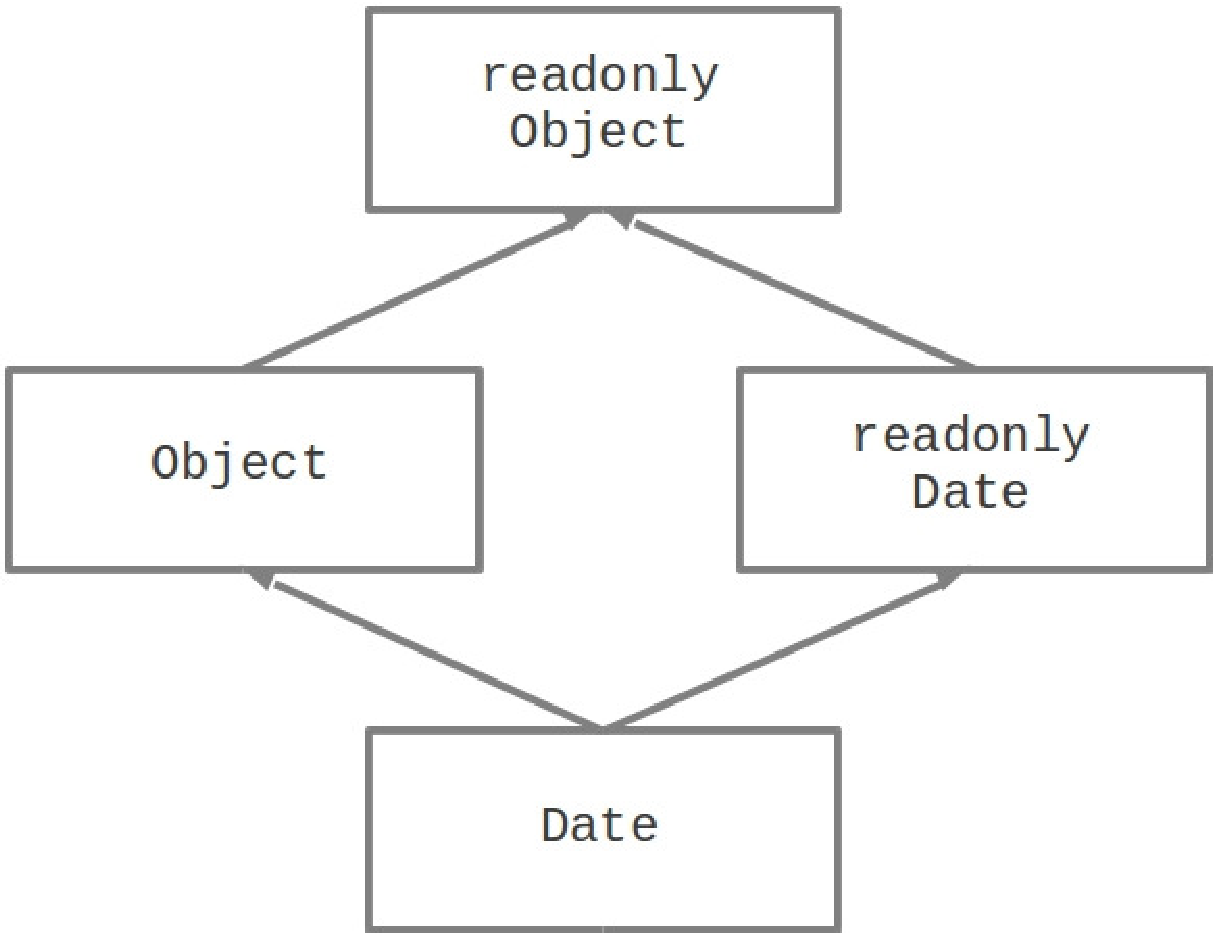
\includegraphics[scale=0.4]{javari_classes.pdf}}
\caption{Фрагмент иерархии классов в Javari}
\label{pic:javari_classes}
\end{figure}

На данном рисунке представлена иерархия типов в Javari. Система типов гарантирует, что изменяющие объект методы не могут быть вызваны на неизменяемых ссылках.

Ключевое слово readonly может быть спользовано при декларации любой переменной, поля, параметра или возвращаемого значения метода. Его также можно применять к неявному параметру this:

\begin{lstlisting}[caption=readonly метод, label=code:readonly_method]
public char charAt(int index) readonly { ... }
\end{lstlisting}

В контексте этого метода this будет неизменяемым.

Модификаторы изменяемости, введенные в Javari не меняют поведения программы во время исполнения. Такой подход обеспечивает обратную совместимость файлов, сгенерированных Javari, с файлами, сгенерированными обычным javac. Одним из последствий такого подходя является то, что два перегруженных метода не могут отличаться только изменяемостью их параметров. Например, такие два метода не могут перегружать друг друга:

\begin{lstlisting}[caption=Перегрузка методов, label=code:javari_method_overloading]
void foo(/*mutable*/ Date d) { ... } 
void foo(readonly Date d) { ... }
\end{lstlisting}

Это аналогично тому, что в Java два перегуженных метода не могут отличаться только типовыми параметрами.

Javari также позволяет исключать некоторые поля из абстрактного состояния объекта. По умолчанию все поля являются частью абстрактного состояния объекта и, соответсвенно, не могу быть изменены через неизменяемую ссылку. Если поле объявлено как assignable, то его значение всегда может быть переприсвоено (даже через read-only ссылку). Ключевое слово mutable означает, что поле может быть изменено даже через неизменяемую ссылку. Это может быть полезно для кэширования данных или, например, для реализации логирования, как в следующем примере:

\begin{lstlisting}[caption=assignable и mutable поля, label=code:assignable_mutable]
class Foo { 
    assignable int hc; 
    final mutable List<String> log = new ArrayList<String>;
    
    int hashCode() readonly { 
        log.add("hashCode invoked");
        if (hc == 0) { 
            hc = ... ;
        } 
        return hc; 
    } 
}
\end{lstlisting}

Javari также позволяет добавлять модификаторы изменяемости к типовым параметрам:

\begin{lstlisting}[caption=Модификаторы изменяемости в типовых параметрах, label=code:javari_generic_local]
/*mutable*/ List</*mutable*/ Date> ld1; // add/remove and mutate elements 
/*mutable*/ List<readonly Date> ld2; // add/remove 
readonly List</*mutable*/ Date> ld3; // mutate elements 
readonly List<readonly Date> ld4; // (neither)
\end{lstlisting} 

Можно представить себе ситуацию, когда программисту захочется управлять изменяемостью типового параметра: например, написать mutable X, где X -- типовый параметр:

\begin{lstlisting}[caption=Модификаторы изменяемости и типовые параметры, label=code:javari_generic_mutable]
class Container<X> {
    void foo() {
       mutable X x = ...;
    }
}
\end{lstlisting} 

Javari запрещает такие типы потому что это не сочетается с подходом к типовым параметрам, принятым в Java, и это может привести к превращении неизменяемой ссылки в изменяемую. Но в Javari, как и в Java, автор класса с типовым параметром может наложить на этот параметр границы. В примере ниже параметр X модет быть readonly Date, mutable Date или каким-либо из их наследников, в то время как Y может быть только mutable Date или его наследником. 

\begin{lstlisting}[caption=Объявление класса с типовыми параметрами, label=code:javari_generic_class]
class Foo<X extends readonly Date, Y extends mutable Date> { ... }
\end{lstlisting} 

Также Javari позволяет абстрагироваться от изменяемости типового параметра. Это можно сделать с помощью конструкции ? readonly C, где С -- какой-то тип. Так, List<? readonly Date> является суперклассом для List<readonly Date> и List<mutable Date>. 

\begin{figure}[h]
\center{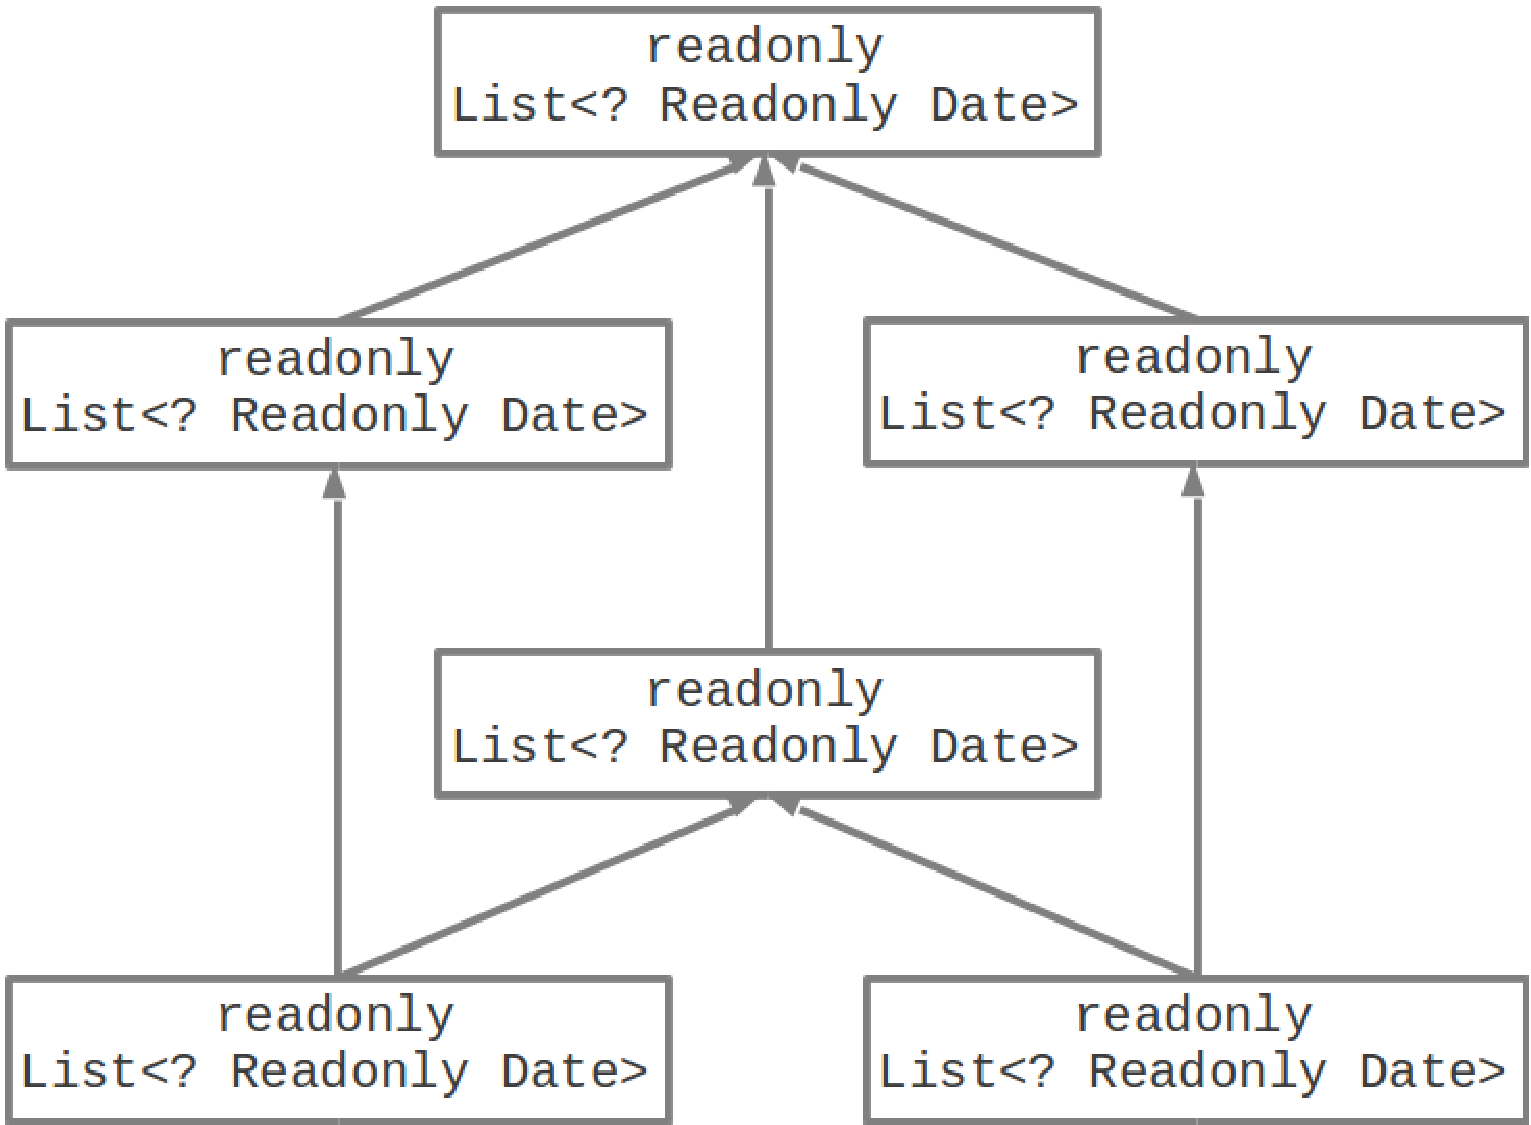
\includegraphics[scale=0.4]{javari_list_classes.pdf}}
\caption{Фрагмент иерархии классов в Javari}
\label{pic:javari_list_classes}
\end{figure}


Наконец, рассмотрим назначение ключевого слова romaybe. Пусть есть класс DateCell, который хранит в себе значение типа Date. Необходимо определить метод getValue, который будет возвращать это значение. Какого модификатор изменяемости должен стоять на возвращаемом значении? Если метод getValue вызывается на изменяемом объекте, то и его результат должен быть изменяемым. Если же он вызван на неизменяемом объекте, и результат его выполнения должен быть неизменяемым. Для решения этой проблемы в Javari было введено еще одно ключевое слово - romaybe. Так будет выглядеть класс DateCell с использованием этого ключевого слова:

\begin{lstlisting}[caption=Ключевое слово romaybe, label=code:javari_romaybe]
class DateCell { Date value; romaybe Date getValue() romaybe { return value; }
}
\end{lstlisting}

В данной ситуации для системы типов существует два метода getValue: в первом все ключевые слова romaybe будут заменены на readonly, а во втором просто опущены. 

Javari предоставляет инструмент под названием Javarifier, позволяющий добавить модификаторы изменяемости к уже существующему коду. На входе он принимает класс-файлы. В начале работы алгоритма некоторые поля помечаются как assignable или mutable (например, на основании того, что они меняются в методе hashCode). Данный алгоритм генерирует и решает систму утверждений для анализируемой программы. Используются два типа утверждений:
\begin{itemize}
	
	\item \textit{некотнтролируемое утверждение} о том, что некая ссылка является неизменяемой: "x is mutable"
	
	\item \textit{контролируемое утверждение} о том, что некая ссылка явлется измеянемой, если другая ссылка является изменяемой: "if y is mutable then x is mutable"
	
\end{itemize}
После составления системы утверждений алгоритм рашает ее.

Минусом данного подхода является то, что в общем случае количество уравнений а данной системе $~O(n^2)$, где n - количесвто ссылок в анализируемом коде. 

\subsection{Immutability Generic Java}

Immutablility Generic Java (IGJ) -- это расширение языка Java, которое позволяет выражать утверждения о неизменяемости объектов без внесения изменений в синтаксис Java, для этого IGJ использует типовые параеметры и аннотации. В IGJ каждый класс имеет дополнительный типовый параметр, который может быть Immutable, Mutable или ReadOnly. IGJ поддерживает как объектную так и ссылочную неизменяемость. IGJ также разрешает ковариантные изменения типовых параметров в безопасной форме, например, неизменяемый список целых чисел является потомком неизменяемого списка чисел.

Рассмотрим применение данного расширения на примере:

\begin{lstlisting}[caption=Ключевое слово romaybe, label=code:igj_graph]
class Edge<I extends ReadOnly> {
    private long id;
    
    @AssignsField Edge(long id) {
        this.setId(id);
    }
    
    @AssignsField synchronized void setId(long id) {
        this.id = id;
    }
    
    @ReadOnly syncronized long getId() {
        return id;
    }
    
    @Immutable long getIdImmutable() {
        return id;
    }
    
    @ReadOnly Edge<I> copy() {
        return new Edge<I>(id);
    }
    
    static void print(Edge<ReadOnly> e) {...}
}

class Graph<I extends ReadOnly> {
    List<I, Edge<I>> edges;
    
    @AssignsField Graph(List<I, Edge<I>> edges) {
        this.edges = edges;
    }
    
    @Mutable void addEdge(Egde<Mutable> e) {
        this.edges.add(e);
    }
    
    static <X extends ReadOnly> Edge<X> 
        findEdge(Graph<X> g, long id) {...}
}
\end{lstlisting}

В примере \ref{code:igj_graph} представлены два IGJ сласса: Edge и Graph. В строчках 1 и 27 определен параметр неизменяемости I. Если в декларации класса отсутсвует дирректива extends, считается, что класс наследует Object<I>. Присваивание this.id = id разрешено, так как метод setId помечен как Mutbale. Метод print, например, принимает любой объект типа Egde, вне зависисмости от его изменяемости. Одним из плюсов IGJ является то, что тот факт, что поля некотго объекта имеют тот же параметр изменяемости, что и сам объект, легко выражается при помощи типовых параметров, как, например это сделано в строке 28. Например, в С++ поля, не обозначенные как const или mutable имеют модификатор неизменяемости такой же, как и у объекта, их содержащего, но при этом отсутсвует возможность указать, что какая-либо локальная переменная, параметр метода или возвращаемое значение имеют такую же неизменяемость, как и объект, на котором данный метод вызван, IGJ же предоставляет такую возможность.

Аннотация @AssignsField решает проблему с изменяемостью this в конструкторе. В контсрукторе неизменяемого объекта нельзя счиать this Mutable, так как в этом случае такая изменяемая ссылка могла бы "утечь". Из метода, проаннотированного как AssignsField ссылка на this может "утечь" только как ReadOnly ссылка. 

Подход, описанный в данной работе, несомненно, позволяет выражать различные утверждения о неизменяемости объектов. Но у него есть несколько минусов:
\begin{itemize}
\item Получающийся код часто выглядит достаточно громоздко.
\item Фаза конструирования объекта заканчивается тогда, когда заканчивает работу его конструктор. Это не позволяет достаточно легко создавать неизменяемые циклические структуры данных. Существующее расширение OIGJ \textit{ссфлка на работу} решает проблему с конструированием объектов, но делает это путем введения понятия владения объектом и, как следствие, добавлением еще одного типового параметра к каждому типу. 
\item Для того, чтобы эффективно использовать уже существующий код из классов, написанных с использованием IGJ необходимо вручную добавить в него дополнительные типовые параметры, отвечающие за изменяемость обхектов
\end{itemize}

\subsection{D}

Подход, похожий на тот, что был описан в IGJ используется в объекно-ориентированном языке D~\footnote{http://dlang.org/}. В D концепции объектной и ссылочной неизменяемости поддерживаются на уровне языка.

Во второй версии этого языка существует два ключевых слова для выражения неизменяемости: const и immutable. Ключевое слово immutable означает, что не существует ссылки, через которую данные могут быть изменены. const обозначает, что по данной ссылке данные менять нельзя, но может существовать ссылка, через которую данные могут быть изменены. 

\begin{lstlisting}[caption=const vs immutable, label=code:d_const_vs_immutable]
int[] foo = new int[5];     // foo is mutable.
const int[] bar = foo;      // bar is a const view of mutable data.
immutable int[] baz = foo;  // Error:  all views of immutable data must be immutable.
 
immutable int[] nums = new immutable(int)[5];  // No mutable reference to nums may be created.
const int[] constNums = nums;                  // Immutable is implicitly convertible to const.
int[] mutableNums = nums;                      // Error:  Cannot create a mutable view of immutable data.
\end{lstlisting}

В отличае от const в C++, const и immutable в D обеспечивают полноценную глубокую неизменяемость, то есть, любые данные, доступные через const или immutbale объект, также константны или неизменяемы, соответсвенно.

\begin{lstlisting}[caption=const vs immutable, label=code:d_const_vs_immutable]
class Foo {
    Foo next;
    int num;
}
 
immutable Foo foo = new immutable(Foo);
foo.next.num = 5;  // Error:  foo.next is of type immutable(Foo).
                   // foo.next.num is of type immutable(int).
\end{lstlisting}

\subsection{Uniqueness and Reference Immutability for Safe Parallelism}

В работе Uniqueness and Reference Immutability for Safe Parallelism представлено расширение для языка C\#. Основной задачей этого расширения является ограничение изменений областей памяти при параллельном программировании. Это достигается компбинацией модификаторов изменяемости и уникальности. Система типов поддерживает полиморфизм относительно этих модификаторов, а также простое создание циклов неизменяемых объектов.

В рамках данной работы у каждой сслки может быть один из следующих модификаторов:
\begin{itemize}
\item writable -- "обычная" ссылка, позволябщая изменять объект, на который она ссылается
\item readable -- неизменяемая ссылка, которая не позволяет изменять объект, на который она ссылается
\item immutbale -- ссылка на неизменяемый объект
\item isolated -- уникальная ссылка на кластер объектов (то есть, все пути в этот подраф объектов извне будут идти через эту ссылку)
\end{itemize}

Введение такого понятия, как isolated ссылка, повзоляет решить проблему с созданием неизменяемых циклических структур данных, так как если некая ссылка явлется едиснвтенной ссылкой на некий подграф объектов, то изменяемость этого подграфа может быть едитновременно безопасно изменена, так как не существует других ссылок на данный подграф. 

В предложенном в данной работе языке отсутсвуют глобальные изменяемые переменные и поля, исключаемые из состояния объекта, что позволяет, напрмиер, говорить о том, что через readable ссылку не может быть достигнута никакая writable ссылка. Подобные ограничения полезны при анализе многопоточного поведения программы, но для статического контроля за изменяемостью они представляются слишком сильными. Например, введение подобный ограничений для Java означало бы отказ от не-final статических полей, а так же от хранения в статических полях объектов, чье стостояние может быть изменено. Также в данной работе никак не рассмотрен вопрос о том, каким образом при наличии всех этих ограниченйи могу бы быть использован уже существующий код.






























\section{Постановка задачи}

Целью данной работы была разработка системы, позволяющей контролировать изменяемость объектов на этапе компиляции для языка Java. 

К данной системе были предъявлены следующие требования:

\begin{itemize}
	\item Должна быть поддержана как объектная, так и ссылочная неизменяемость.
	
	\item Негобходима возможность исключать некоторые поля из абстрактного состояния объекта. 
	
	\item Данная система должна давать возможность создавать неизменяемые циклические структуры объектов.
	
	\item Необходимо иметь вохможность использовать уже существующий код.
\end{itemize}

В рамках данной работы решались следующие задачи:

\begin{itemize}

	\item Разработка системы аннотаций, позволяющей выражать неизменяемость объектов.
	
	\item Разработка алгоритма вывода аннотаций для существующего кода.

\end{itemize}



